\section{DCT}

\subsection{Transformadas de comprimento finito}

\begin{frame}%[allowframebreaks]
  \frametitle{Transformadas de comprimento finito}
  Equação de análise:
  \begin{equation}
  A[k] = \sum_{n=0}^{N-1} x[n] \phi^{\ast}_{k} [n]
  \end{equation}

  Equação de síntese:
  \begin{equation}
  x[n] = \frac{1}{N} \sum_{k=0}^{N-1} A[k] \phi_k[n]
  \end{equation}

  As sequências $\phi_k [n]$ são chamadas de \textbf{sequências de base} e são ortogonais entre si, i.e.
  \begin{equation}
  \langle \phi_k , \phi_m \rangle = \frac{1}{N} \sum_{n=0}^{N-1} \phi_k [n] \phi^{\ast}_m [n] = \begin{cases} 1, \quad m=k \\ 0, \quad m \neq k .\end{cases} = \delta_{m,k}.
  \end{equation}
\end{frame}


\subsection{Discrete Time Fourier Transform (DFT)}
\begin{frame}%[allowframebreaks]
  \frametitle{Discrete Time Fourier Transform (DFT)}
  Para a DFT temos
  \begin{equation}
   \phi_k [n] = e^{j \frac{2 \pi kn}{N}}
  \end{equation}

  Existem $N$ exponencias complexas distintas: $\phi_0, \phi_1, \ldots, \phi_{N-1}$.

  $\{ \phi_k \}_{k \in [0,N-1]}$ forma uma base para o espaço das sequências de tamanho $N$.

  \begin{equation}
  x[n] \mathrel{\mathop{\rightleftarrows}^{\mathrm{DFT}}_{\mathrm{iDFT}}} X[k]
  \end{equation}

  Se $x[n]$ é real, então $X[k]$ é par e complexo.
\end{frame}

\begin{frame}%[allowframebreaks]
  \frametitle{Outras Transformadas}
  Existe uma base $\{ \phi_k \}$ tal que sendo $x[n]$ real teremos $X[k]$ também real?

  \vspace{0.5cm}
  \begin{itemize}
  \item Transformada Haar
  \item Transformada Hadamard
  \item Transformada Hartley
  \item Transformada Discreta em Cossenos
  \end{itemize}
\end{frame}


\subsection{Transformada Discreta em Cossenos (DCT)}
\begin{frame}%[allowframebreaks]
  \frametitle{Definição da DCT}
  \begin{itemize}
  \item As sequências de base $\phi_k$ são cossenos.
  \item Cossenos são funções periódicas com simetria par.
  \item A extensão de $x[n]$ fora do intervalo $0 \leq n \leq (N-1)$ na equação
          \begin{equation}
          x[n] = \frac{1}{N} \sum_{k=0}^{N-1} A[k] \phi_k[n]
          \end{equation}
        será periódica e com simetria par.
  \item sequência finita $\rightarrow$ sequência periódica
  \item sequência periódica $\rightarrow$ sequência finita
  \item Existem 8 formas diferentes de fazer a extensão periódica de uma sequência.
        \begin{itemize}
        \item borda esquerda/direita; simetria par/ímpar; ponto dos dados/ponto intermediário
        \end{itemize}
  \end{itemize}
\end{frame}

\begin{frame}%[allowframebreaks]
  \frametitle{Simetrias}
    \vspace{-0.2cm}
    \begin{figure}[ht]
    \centering
    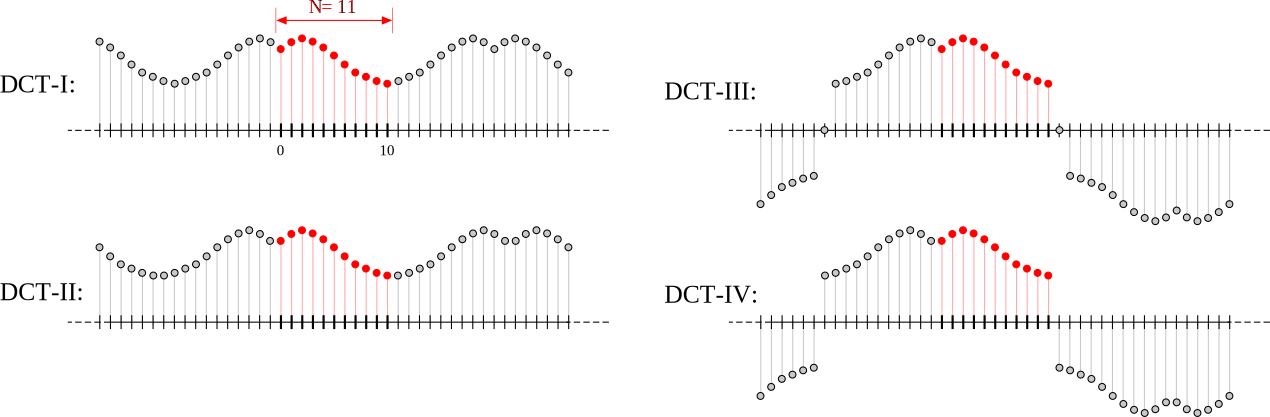
\includegraphics[width=\textwidth]{images/DCT-symmetries.pdf}
    \caption{Extensão par e ímpar na definição dos tipos de DCT. (Wikipedia)}
    \label{fig:DCT-symmetries}
    \end{figure}
\end{frame}

\begin{frame}%[allowframebreaks]
  \frametitle{DCT-I}
    \begin{figure}[ht]
    \centering
    \includegraphics[width=0.4\textwidth]{images/dct-1-ex.pdf}
    \label{fig:DCT-I}
    \end{figure}
    $\tilde{x_1}[n]$ possui período $(2N-2)$ e possui simetria par em torno de $n=0$ e $n=(N-1)$.
\end{frame}

\begin{frame}%[allowframebreaks]
  \frametitle{DCT-II}
    \begin{figure}[ht]
    \centering
    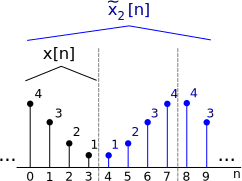
\includegraphics[width=0.4\textwidth]{images/dct-2-ex.pdf}
    \label{fig:DCT-II}
    \end{figure}
    $\tilde{x_2}[n]$ possui período $2N$ e possui simetria par em torno de $n=-1/2$ e $n=N-1/2$.
\end{frame}

\begin{frame}%[allowframebreaks]
  \frametitle{DCT-III}
    \vspace{-0.2cm}
    \begin{figure}[ht]
    \centering
    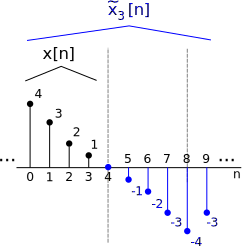
\includegraphics[width=0.4\textwidth]{images/dct-3-ex.pdf}
    \label{fig:DCT-III}
    \end{figure}
    $\tilde{x_3}[n]$ possui período $4N$ e possui simetria par em torno de $n=0$ e ímpar em torno de $n=N$.
\end{frame}

\begin{frame}%[allowframebreaks]
  \frametitle{DCT-IV}
    \vspace{-0.2cm}
    \begin{figure}[ht]
    \centering
    \includegraphics[width=0.4\textwidth]{images/dct-4-ex.pdf}
    \label{fig:DCT-IV}
    \end{figure}
    $\tilde{x_4}[n]$ possui período $4N$ e possui simetria par em torno de $n=-1/2$ e ímpar em torno de $n=N-1/2$.
\end{frame}


\subsection{DCT-I}
\begin{frame}[allowframebreaks]
  \frametitle{DCT-I}
    \begin{figure}[ht]
    \centering
    \includegraphics[width=0.4\textwidth]{images/dct-1-ex.pdf}
    \label{fig:DCT-I-a}
    \end{figure}
    $\tilde{x_1}[n]$ possui período $(2N-2)$ e possui simetria par em torno de $n=0$ e $n=(N-1)$.

        \begin{equation}
        \tilde{x_1}[n] = x_{\alpha} \left[ ((n))_{2N-2} \right] + x_{\alpha} \left[ ((-n))_{2N-2} \right]
        \end{equation}
        onde $((n))_N$ significa $n \mod N$, e a sequência modificada é definida por $x_{\alpha}[n] = \alpha[n] x[n]$, com
        \begin{equation}
        \alpha[n] = \begin{cases} \frac{1}{2} , \quad n = 0 \text{ e } N-1, \\
                                1, \quad 1 \leq n \leq N-2 .\end{cases}
        \end{equation}

  \framebreak
    \begin{figure}[ht]
    \centering
    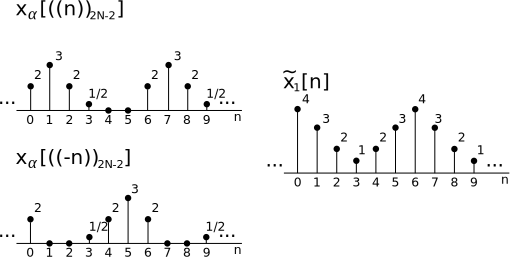
\includegraphics[width=0.8\textwidth]{images/dct-1-parts.pdf}
    \label{fig:DCT-I-parts}
    \end{figure}
  \framebreak

  \begin{itemize}
  \item $\tilde{x_1}[n]$ possui período igual a $2N-2$.
  \item base de cossenos harmonicamente relacionados, $\omega_0 = 2\pi/(2N-2)$, teremos: $\cos\left(\frac{2\pi k n}{2N-2} \right) = \cos\left(\frac{ \pi k n}{N-1}\right)$.
  \end{itemize}
  \begin{eqnarray}
  X[k] &=& \sum_{n=0}^{2N-3} \tilde{x_1}[n] \cos\left( \frac{\pi k n}{N-1} \right) \\
        &=& \tilde{x_1}[0] \cos(0) + \sum_{n=1}^{N-2} \tilde{x_1}[n] \cos\left( \frac{\pi k n}{N-1} \right)  \\
        && + \tilde{x_1}[N-1] \cos\left( \frac{\pi k (N-1)}{N-1} \right) + \sum_{n=N}^{2N-3} \tilde{x_1}[n] \cos\left( \frac{\pi k n}{N-1} \right) \nonumber 
  \end{eqnarray}

  \framebreak

  fazendo $n' = 2N-2-n$  no segundo somatório teremos
  \begin{eqnarray}
  X[k] &=& \ldots \nonumber \\
        && \tilde{x_1}[0] \cos(0) + \sum_{n=1}^{N-2} \tilde{x_1}[n] \cos\left( \frac{\pi k n}{N-1} \right)  \\
        && + \tilde{x_1}[N-1] \cos\left( \frac{\pi k (N-1)}{N-1} \right) \nonumber \\
        && + \sum_{n'=N-2}^{1} \underbrace{\tilde{x_1}[2N-2-n']}_{ \underset{\tilde{x_1} \text{ é par }}{ = \tilde{x_1}[n] = \tilde{x_1}[n']} } \cos\left( \frac{\pi k (2N-2-n')}{N-1} \right) \nonumber
  \end{eqnarray}

  \framebreak

  Iremos utilizar $\cos(A+B) = \cos A \cos B - \sin A \sin B$

  \begin{eqnarray}
  \cos\left( \frac{\pi k (2N-2-n')}{N-1} \right) &=& \underbrace{\cos\left( \frac{\pi k (2N-2)}{N-1} \right)}_{=1} \cos\left( \frac{-n' k \pi}{N-1} \right) \nonumber \\
        && -  \underbrace{\sin\left( \frac{\pi k (2N-2)}{N-1} \right)}_{=0} \sin\left( \frac{-n' k \pi}{N-1} \right) \nonumber \\
        &=& \cos\left( \frac{n' k \pi}{N-1} \right)
  \end{eqnarray}

  \framebreak

  \begin{eqnarray}
  X[k] &=& \ldots \nonumber \\ 
        && \tilde{x_1}[0] \cos(0) + \sum_{n=1}^{N-2} \tilde{x_1}[n] \cos\left( \frac{\pi k n}{N-1} \right)  \\
        && + \tilde{x_1}[N-1] \cos\left( \frac{\pi k (N-1)}{N-1} \right) \nonumber \\
        && \sum_{n'=1}^{N-2} \tilde{x_1}[n'] \cos\left( \frac{n' k \pi}{N-1} \right) \\
        &=& 2 \sum_{n=0}^{N-1} \alpha[n] x[n] \cos \left( \frac{\pi k n}{N - 1} \right)
  \end{eqnarray}

  \framebreak

  A DCT-I é definida pelo par de transformada:
  \begin{equation}
  X^{C1}[k] = 2 \sum_{n=0}^{N-1} \alpha[n] x[n] \cos \left( \frac{\pi k n}{N - 1} \right) , \quad 0 \leq k \leq N-1 ,
  \end{equation}
  \begin{equation}
  x[n] = \frac{1}{N-1} \sum_{k=0}^{N-1} \alpha[k] X^{C1}[k] \cos \left( \frac{\pi k n}{N - 1} \right) , \quad 0 \leq n \leq N-1.
  \end{equation}
\end{frame}



\subsection{DCT-II}
\begin{frame}[allowframebreaks]
  \frametitle{DCT-II}
    \begin{figure}[ht]
    \centering
    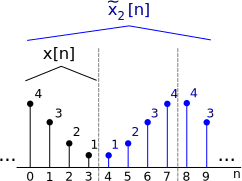
\includegraphics[width=0.4\textwidth]{images/dct-2-ex.pdf}
    \label{fig:DCT-II-a}
    \end{figure}
    $\tilde{x_2}[n]$ possui período $2N$ e possui simetria par em torno de $n=-1/2$ e $n=N-1/2$.

    $x[n]$ é estendido para ter período $2N$, sendo a sequência periódica dada por
        \begin{equation}
        \tilde{x_2}[n] = x \left[ ((n))_{2N} \right] + x \left[ ((-n-1))_{2N} \right]
        \end{equation}

        \framebreak

        A DCT-II é definida pelo par de transformada:
        \begin{equation}
        X^{C2}[k] = 2 \sum_{n=0}^{N-1} x[n] \cos \left( \frac{\pi k (2n+1)}{2N} \right), \quad 0 \leq k \leq N-1 .
        \end{equation}

        \begin{equation}
        x[n] = \frac{1}{N} \sum_{k=0}^{N-1} \beta[k] X^{C2}[k] \cos \left( \frac{\pi k (2n+1)}{2N} \right), \quad 0 \leq n \leq N-1 .
        \end{equation}
        onde a função de peso $\beta[k]$ é dada por
        \begin{equation}
        \beta[k] = \begin{cases} \frac{1}{2} , \quad k = 0 \\ 1 , \quad 1 \leq k \leq N - 1 . \end{cases}
        \end{equation}

        \framebreak
        Muitas vezes inclui-se um fator de normalização para tornar a transformada unitária, ou seja,
        deverá ser ortonormal e terá a propriedade $\sum_{n=0}^{N-1} \left( x[n] \right)^2 = \sum_{k=0}^{N-1} \left( X^{C2} [k] \right)^2$.

        \begin{equation}
        \tilde{X}^{C2}[k] = \sqrt{\frac{2}{N}} \tilde{\beta}[k] \sum_{n=0}^{N-1} x[n] \cos \left( \frac{\pi k (2n+1)}{2N} \right), \quad 0 \leq k \leq N-1 .
        \end{equation}

        \begin{equation}
        x[n] = \sqrt{\frac{2}{N}} \sum_{k=0}^{N-1} \tilde{\beta}[k] \tilde{X}^{C2}[k] \cos \left( \frac{\pi k (2n+1)}{2N} \right), \quad 0 \leq n \leq N-1 .
        \end{equation}
        onde a função de peso $\tilde{\beta}[k]$ é dada por
        \begin{equation}
        \tilde{\beta}[k] = \begin{cases} \frac{1}{\sqrt{2}} , \quad k = 0 \\ 1 , \quad 1 \leq k \leq N - 1 . \end{cases}
        \end{equation}
\end{frame}


\begin{frame}[allowframebreaks]
  \frametitle{Forma Matricial}

  Para $0 \leq k \leq N-1$m temos
  \begin{eqnarray}
  \tilde{X}^{C2}[k] &=& \sqrt{\frac{2}{N}} \tilde{\beta}[k] \sum_{n=0}^{N-1} x[n] \cos \left( \frac{\pi k (2n+1)}{2N} \right) \\
        &=& \sum_{n=0}^{N-1} x[n]  \sqrt{\frac{2}{N}}  \tilde{\beta}[k] \cos \left( \frac{\pi k (2n+1)}{2N} \right) \\
        &=& \sum_{n=0}^{N-1} x[n] c[k,n]
  \end{eqnarray}
  onde definimos
  \begin{equation}
  c[k,n] \triangleq \sqrt{\frac{2}{N}}  \tilde{\beta}[k] \cos \left( \frac{\pi k (2n+1)}{2N} \right) \quad  k,n = 0,1,\ldots,N-1
  \end{equation}

  Temos então a matriz $N \times N$ da transformada em cossenos
  \begin{equation}
  \left[ \begin{array}{ccc} \cdots & \cdots & \cdots \\
  \cdots & c[n,m] & \cdots \\ \cdots & \cdots & \cdots \end{array} \right]
  =\left[ \begin{array}{c} {\bf c}_0^T \\ \cdots \\ {\bf c}_{N-1}^T \end{array} \right]
  ={\bf C}^T
  \end{equation}

   ${\bf c}_i^T=[c[i,0],\cdots,c[i,N-1]$ é a $i$-ésima linha da matriz de DCT ${\bf C}$.
   Estes vetores linha são ortonormais:
  \begin{equation}
  \langle {\bf c}_i,{\bf c}_j \rangle = {\bf c}_i^T {\bf c}_j =\delta_{ij}
  =\left\{ \begin{array}{ll}1 & i=j \\ 0 & i\ne j \end{array} \right.
  \end{equation}
  então a matriz ${\bf C}$ é ortonormal
  \begin{equation}
  {\bf C}^{-1}={\bf C}^T,\;\;\;\;\mbox{i.e.} \;\;\;\;{\bf C}^T {\bf C}= {\bf I} 
  \end{equation}
  e real ${\bf C}={\bf C}^*$. A DCT sobre $x[n] = {\bf x}$ pode ser expressa na forma matricial
  \begin{equation}
  {\bf X}={\bf C}^T {\bf x}
  \end{equation}
\end{frame}

\begin{frame}[allowframebreaks]
  \frametitle{DCT 2D}

  Considere uma imagem $N \times N$, $\mathbf{A}$.
  A 2D-DCT de $\mathbf{A}$ é dada por $\mathbf{Y} = \mathbf{C} \mathbf{X} \mathbf{C}^T$, e a
  inversa é $\mathbf{X} = \mathbf{C}^T \mathbf{Y} \mathbf{C}$.

  \framebreak

    \begin{figure}[ht]
    \centering
    \includegraphics[width=0.95\textwidth]{images/ex-num-dct.png}
    \caption{Exemplo DCT.}
    \label{fig:dct_2d_ex}
    \end{figure}

\end{frame}


\subsection{Relação entre DCT-I e DFT}
\begin{frame}[allowframebreaks]
  \frametitle{Relação entre DCT-I e DFT}

        \begin{equation}
        \tilde{x_1}[n] = x_{\alpha} \left[ ((n))_{2N-2} \right] + x_{\alpha} \left[ ((-n))_{2N-2} \right]
        \end{equation}
        $\tilde{x_1}[n]$ é construído a partir de $x[n]$ e $\alpha[n]$. Podemos definir uma sequência finita $x_1[n]$ com
        base na sequência periódica $\tilde{x_1}[n]$:
        \begin{equation}
        x_1 [n] = x_{\alpha} \left[ ((n))_{2N-2} \right] + x_{\alpha} \left[ ((-n))_{2N-2} \right] = \tilde{x_1}[n], \quad n = 0, 1, \ldots, 2N-3.
        \end{equation}

        \framebreak
        A DFT da sequência $x_1 [n]$ com $(2N-2)$ pontos é dada por
        \begin{eqnarray}
        X_1[k] &=& \mathrm{DFT}\{x_1[n]\} \\
                &=& \mathrm{DFT}\{x_{\alpha} \left[ ((n))_{2N-2} \right]\} + \mathrm{DFT}\{x_{\alpha} \left[ ((-n))_{2N-2} \right]\} \\
                &=& X_\alpha [k] + X_\alpha^\ast [k] \\
                &=& 2 \mathit{Re} \{ X_\alpha [k] \} , \quad k = 0, 1, \ldots, 2N -3 \\
                &=& 2 \sum_{n=0}^{N-1} \alpha[n] x[n] \cos \left( \frac{2 \pi k n}{2N-2} \right) = X^{C1}[k].
        \end{eqnarray}
        $X_\alpha [k]$ é a DFT de $(2N-2)$ pontos da sequência $\alpha[n]x[n]$ de $N$ pontos, ou seja, devemos
        preencher $\alpha[n]x[n]$ com $(N-2)$ zeros.

        Então a DCT-I de uma sequência de $N$ pontos é idêntica à DFT de $(2N-2)$ pontos da sequência estendida $x_1[n]$,
        e também idêntica à duas vezes a parte real dos primeiros $N$ pontos da DFT de $(2N-2)$ pontos da sequência $x_\alpha [n]$.


        A DCT é $O(N^2)$, enquanto a DFT possui um algoritmo rápido (FFT) $O(N \log N)$.
        Poderemos utilizar a FFT para calcular $X_\alpha[k]$ ou $X_1[k]$ e desta forma teremos uma forma mais
        conveniente para computar a DCT-I.

        Como a DCT-I envolve apenas coeficientes reais, existem também algoritmos eficientes para calcular a DCT-I
        de sequências reais de forma direta, sem a necessidade de multiplicações e adições de números complexos
        \cite{ahmed1974,chen1977}.

        \framebreak
        A DCT-I inversa também pode ser calcular através da DFT inversa, para tanto, iremos construir $X_1[k]$
        a partir de $X^{C1}[k]$ e então calcular a DFT inversa de $(2N-2)$ pontos.
        \begin{equation}
        X_1 [k] = \begin{cases} X^{C1}[k], \quad k = 0, \ldots, N-1 \\ 
                                X^{C1}[2N-2-k], \quad k = N, \ldots, 2N-3. \end{cases}
        \end{equation}
        Utilizando a DFT inversa de $(2N-2)$ pontos teremos
        \begin{equation}
        x_1[n] = \frac{1}{2N-2} \sum_{k=0}^{2N-3} X_1[k] e^{j 2 \pi kn/(2N-2)} , \quad n = 0, 1, \ldots, 2N-3.
        \end{equation}
\end{frame}


\subsection{Relação entre DCT-II e DFT}
\begin{frame}[allowframebreaks]
  \frametitle{Relação entre DCT-II e DFT}

    \begin{figure}[ht]
    \centering
    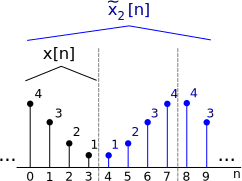
\includegraphics[width=0.4\textwidth]{images/dct-2-ex.pdf}
    \label{fig:DCT-II-a}
    \end{figure}

  Podemos construir $x_2 [n]$ a partir de um período de $\tilde{x}_2[n]$.
  \begin{equation}
  x_2 [n] = x\left[ ((n))_{2N} \right] + x\left[ ((-n-1))_{2N} \right] = \tilde{x}_2[n] , \quad n = 0, 1, 2, \ldots, 2N-1.
  \end{equation}

  \framebreak
  $X_2[k]$ é a DFT de $2N$ pontos de $x_2 [n]$,
  \begin{equation}
  X_2[k] = X[k] + X^\ast [k] e^{j \frac{2 \pi k}{2N}} , \quad k = 0,1, \ldots, 2N-1,
  \end{equation}
  onde $X[k]$ é a DFT de $2N$ pontos da sequência $x[n]$ de $N$ pontos, ou seja, $x[n]$ deve ser estendido com $N$ zeros.


  \framebreak

  \begin{eqnarray}
  X_2[k] &=& X[k] + X^\ast[k] e^{j \frac{2 \pi k}{2N}} \\
        &=& e^{j \frac{\pi k}{2N}} \left( X[k] e^{-j \frac{\pi k}{2N}} + X^\ast[k] e^{j \frac{\pi k}{2N}} \right) \\
        &=& e^{j \frac{\pi k}{2N}} 2 \Re \left\{ X[k] e^{-j \frac{\pi k}{2N}} \right\}
  \end{eqnarray}

  A DFT de $X[k]$ ($2N$ pontos, com $N$ zeros) é dada
  \begin{eqnarray}
  X[k] &=& \sum_{n=0}^{2N-1} x[n] e^{-j \frac{2 \pi kn}{2N}} \\
        && \text{como $x[n]$ foi estendido com $N$ zeros} \\
        &=& \sum_{n=0}^{N-1} x[n] e^{-j \frac{\pi kn}{N}}
  \end{eqnarray}
  Substituindo na equação de $X_2[k]$, teremos
  \begin{eqnarray}
  X_2[k] &=& e^{j \frac{\pi k}{2N}} 2 \Re \left\{ X[k] e^{-j \frac{\pi k}{2N}} \right\} \\
        &=& e^{j \frac{\pi k}{2N}} 2 \Re \left\{ \sum_{n=0}^{N-1} x[n] e^{-j \frac{\pi kn}{N}} e^{-j \frac{\pi k}{2N}} \right\} \\
        &=& e^{j \frac{\pi k}{2N}} 2 \Re \left\{ \sum_{n=0}^{N-1} x[n] e^{-j \frac{\pi k (2n+1)}{2N}} \right\} \\
        &=& e^{j \frac{\pi k}{2N}} \underbrace{ 2 \sum_{n=0}^{N-1} x[n] \cos \left( \frac{\pi k (2n+1)}{2N} \right) }_{X^{C2}[k]}
  \end{eqnarray}
  onde utilizamos o fato de que $x[n]$ é real.

  Concluímos então que
  \begin{equation}
  X^{C2}[k] = 2 \Re \left\{ X[k] e^{-j \frac{\pi k}{2N}} \right\} , \quad k=0,1,\ldots,N-1.
  \end{equation}
  onde $X[k]$ é a DFT de $2N$ pontos de $x[n]$ estendido com $N$ zeros.
  Ou então, utilizando que $X_2[k] = e^{j \frac{\pi k}{2N}} 2 \Re \left\{ X[k] e^{-j \frac{\pi k}{2N}} \right\}$, poderemos escrever
  \begin{equation}
  X^{C2}[k] = e^{-j \frac{\pi k}{2N}} X_2[k] , \quad k=0,1,\ldots,N-1 ,
  \end{equation}
  ou seja, $X^{C2}[k]$ pode ser obtido através da DFT de $2N$ pontos de $x_2[n]$, a extensão simétrica par de $x[n]$.

  \begin{itemize}
  \item Podemos utilizar a FFT para calcular a DFT, e assim poderemos também calcular a DCT-II através da FFT.
  \item Também é possível calcular a inversa da DCT-II utilizando a iFFT (FFT inversa).
  \item Embora a complexidade da aplicação direta da fórmula da DCT requereria $O(N^2)$ operações, é possível utilizar a
        transformada rápida de Fourier (FFT), cuja complexidade é $O(N \log N)$, e calcular a DCT através da FFT com um
        pré- e pós-processamento de $O(N)$ operações.
  \end{itemize}

\end{frame}

\subsection{Propriedade de Compactação de Energia}
\begin{frame}[allowframebreaks]
  \frametitle{Compactação de Energia na DCT-II}
  É preferida a utilização da DCT-II em diversas aplicações de compressão de dados em detrimento da DFT pois
  aquela possui a propriedade de compactação de energia. A DCT-II de uma sequência finita usualmente possui
  coeficientes mais concentrados do que a DFT. A importância disso segue do teorema de Parseval que, para a DCT-II é
  \begin{equation}
  \sum_{n=0}^{N-1} \vert x[n] \vert^2 = \frac{1}{N} \sum_{k=0}^{N-1} \beta[k] \vert X^{c2}[k] \vert^2
  \end{equation}
  onde
  \begin{equation}
  \beta[k] = \begin{cases} \frac{1}{2} , \quad k=0 \\ 1 , \quad 1 \leq k \leq N-1 \end{cases}
  \end{equation}

    \begin{figure}[ht]
    \centering
    \includegraphics[width=0.5\textwidth]{images/compact_energy.png}
    \caption{Efeito de compactação de energia da DCT.}
    \label{fig:compact_energy}
    \end{figure}

\end{frame}

\begin{frame}%[allowframebreaks]
  \frametitle{Notebook DCT - GNU Octave}
  \centering
  \includegraphics[width=0.4\textwidth]{images/qrcode-jupyter-dct.pdf}

  \url{https://nbviewer.jupyter.org/github/leolca/notebooks/blob/master/aev/DCT.ipynb}
\end{frame} 

